\documentclass[tikz,border=6pt]{standalone}
\usepackage{amsmath}
\usepackage{lmodern}
\usepackage{helvet}
\usetikzlibrary{arrows.meta}
\definecolor{input}{HTML}{F8CEAD}
\definecolor{response}{HTML}{C5DFB3}
\definecolor{grid}{HTML}{ADC9E2}
\definecolor{gridtext}{HTML}{355F97}
\definecolor{gridarrow}{HTML}{4875BC}
\definecolor{flow}{HTML}{7EAF51}
\definecolor{inputarrow}{HTML}{EBA875}
\begin{document}
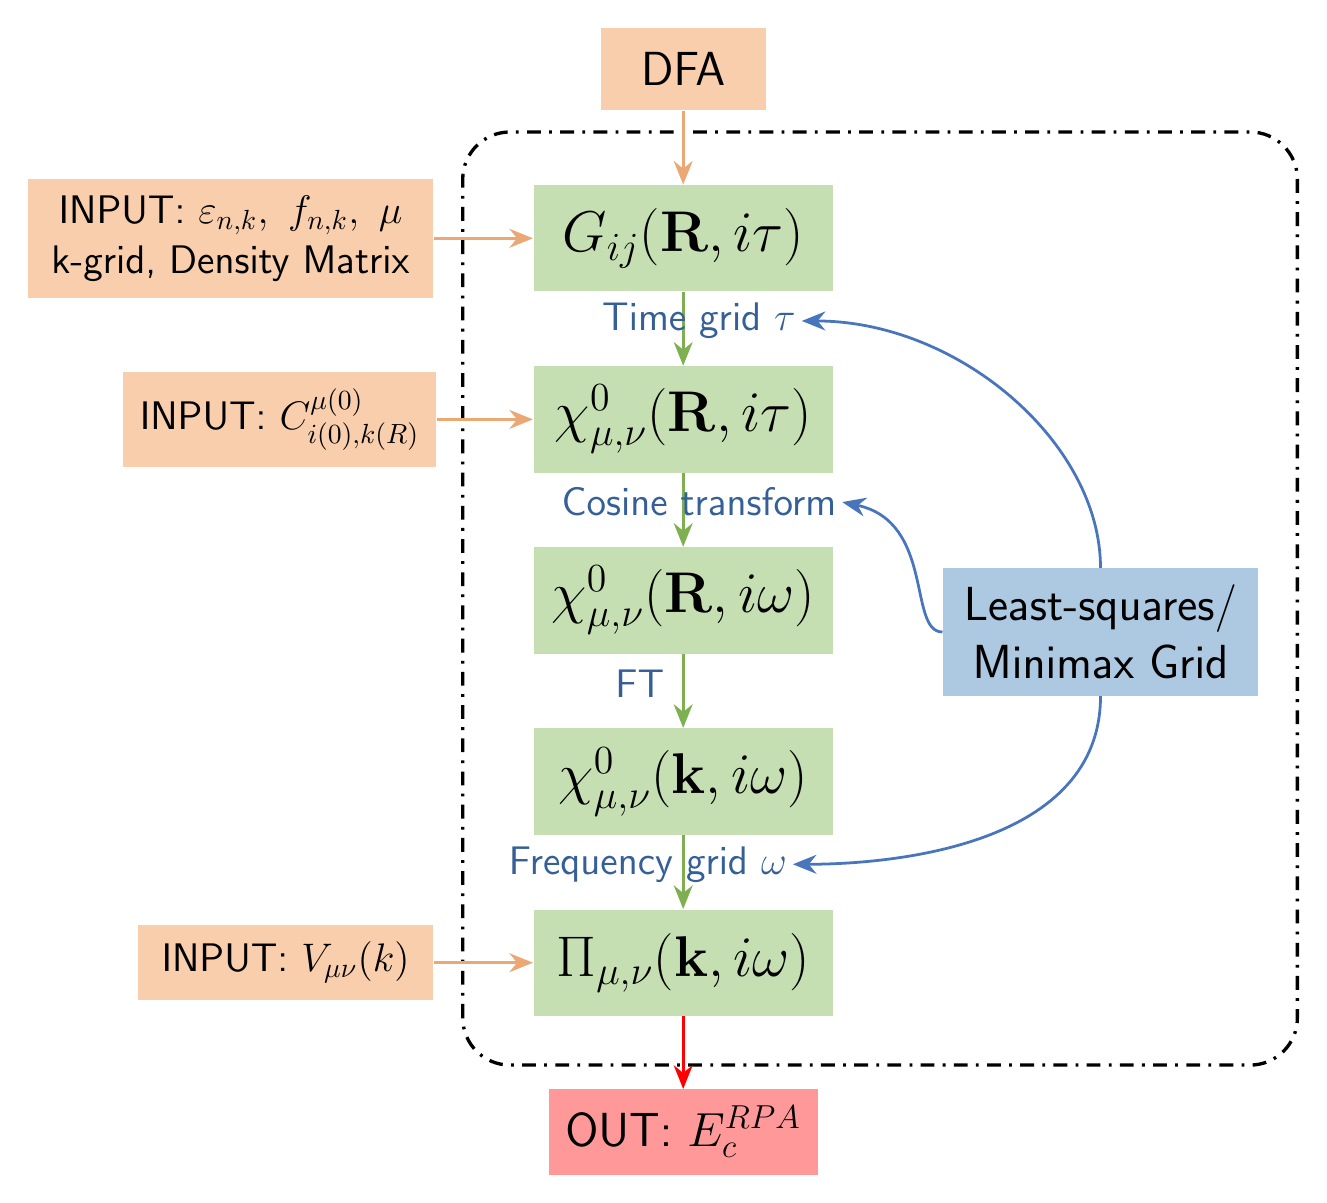
\begin{tikzpicture}[
  font=\sffamily\Large,
  box/.style={align=center,inner sep=6pt},
  quantity/.style={box,fill=response,minimum width=3.8cm,
    minimum height=1.35cm,font=\fontsize{20}{24}\selectfont},
  arrow/.style={-{Stealth[length=3mm,width=2.4mm]},line width=1pt},
  label/.style={text=gridtext,inner sep=2pt}]

\draw[line width=1.2pt,rounded corners=6mm,
  dash pattern=on 5pt off 3pt on 1pt off 3pt]
  (5.8,1.5) rectangle (16.4,13.35);

\node[box,fill=input,minimum width=2.1cm,minimum height=1.05cm,
  font=\sffamily\LARGE] (dfa) at (8.6,14.15) {DFA};
\node[quantity] (g) at (8.6,12.0) {$G_{ij}(\mathbf{R},i\tau)$};
\node[quantity] (chit) at (8.6,9.7) {$\chi^0_{\mu,\nu}(\mathbf{R},i\tau)$};
\node[quantity] (chiw) at (8.6,7.4) {$\chi^0_{\mu,\nu}(\mathbf{R},i\omega)$};
\node[quantity] (chik) at (8.6,5.1) {$\chi^0_{\mu,\nu}(\mathbf{k},i\omega)$};
\node[quantity] (pi) at (8.6,2.8) {$\Pi_{\mu,\nu}(\mathbf{k},i\omega)$};
\node[box,fill=red!40,minimum height=1cm,font=\sffamily\LARGE]
  (out) at (8.6,0.65) {OUT: $E_c^{RPA}$};

\draw[arrow,inputarrow] (dfa) -- (g);
\draw[arrow,flow] (g) -- (chit);
\draw[arrow,flow] (chit) -- (chiw);
\draw[arrow,flow] (chiw) -- (chik);
\draw[arrow,flow] (chik) -- (pi);
\draw[arrow,red] (pi) -- (out);

\node[label] (time) at (8.8,10.95) {Time grid $\tau$};
\node[label] (cosine) at (8.8,8.65) {Cosine transform};
\node[label] at (8.05,6.35) {FT};
\node[label] (frequency) at (8.15,4.05) {Frequency grid $\omega$};

\node[box,fill=input,minimum width=5.15cm,minimum height=1.45cm]
  (bands) at (2.85,12.0)
  {INPUT: $\varepsilon_{n,k},\ f_{n,k},\ \mu$\\k-grid, Density Matrix};
\node[box,fill=input,minimum width=3.9cm,minimum height=1.1cm]
  (coeff) at (3.475,9.7) {INPUT: $C^{\mu(0)}_{i(0),k(R)}$};
\node[box,fill=input,minimum width=3.75cm,minimum height=.9cm]
  (coulomb) at (3.55,2.8) {INPUT: $V_{\mu\nu}(k)$};
\draw[arrow,inputarrow] (bands) -- (g);
\draw[arrow,inputarrow] (coeff) -- (chit);
\draw[arrow,inputarrow] (coulomb) -- (pi);

\node[box,fill=grid,minimum width=4cm,minimum height=1.6cm,
  font=\sffamily\fontsize{16}{21}\selectfont] (grids) at (13.9,7.0)
  {Least-squares/\\Minimax Grid};
\draw[arrow,gridarrow] (grids.north)
  .. controls (13.9,9.4) and (12.1,10.95) .. (time.east);
\draw[arrow,gridarrow] (grids.west)
  .. controls (11.45,7.0) and (11.8,8.4) .. (cosine.east);
\draw[arrow,gridarrow] (grids.south)
  .. controls (13.9,4.3) and (11.3,4.05) .. (frequency.east);
\end{tikzpicture}
\end{document}
